\chapter{Microbit V1 data logging}
Datalogging with a V2 microbit is relatively easy all the details are available here: \url{https://microbit.org/get-started/user-guide/data-logging/} to get started. 

But what about the older V1 can it do it?
\section{Why?}
Often we need applications that allow collection of data over time, for example temperature or light levels through the day. Allowing us potentially analyse the data for trends. The microbit is a fantastic tool with some of these sensors already in place (e.g. light and temperature) or can be added to with extra sensors from add-on boards (such as Kitronik Air Quality and Environmental Board for micro:bit \url{https://shop.pimoroni.com/products/kitronik-air-quality-and-environmental-board-for-micro-bit?variant=39475687227475} )



The answer is yes but it is a little more work and is generally a little more limited but still very worth while. In this article we are going to look at doing this.

\section{Basics}
Ok lets start
\subsection{Building it}
In Figure 1 starting the process off in MakeCode (\url{https://makecode.microbit.org/#editor}) is shown below. Basic mechanism every 1sec 
-	The light level is write from the microbit to the computer (via the USB) a value at a time – serially
-	Same thing will be done for temperature
That is it to start with.
\begin{figure}
    \centering
    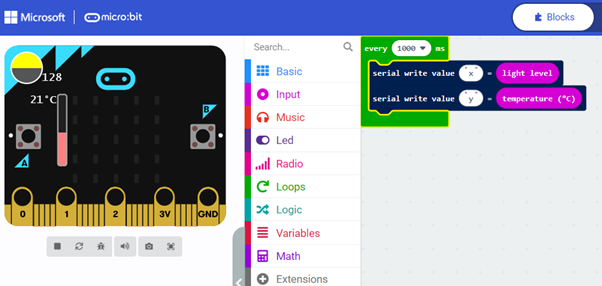
\includegraphics[width=10cm]{chapters/ChapterP2-datalog/figures/datalog1.png}
    \caption{Code for data logging}
    \label{fig:datalog1}
\end{figure}
 
\begin{figure}
    \centering
    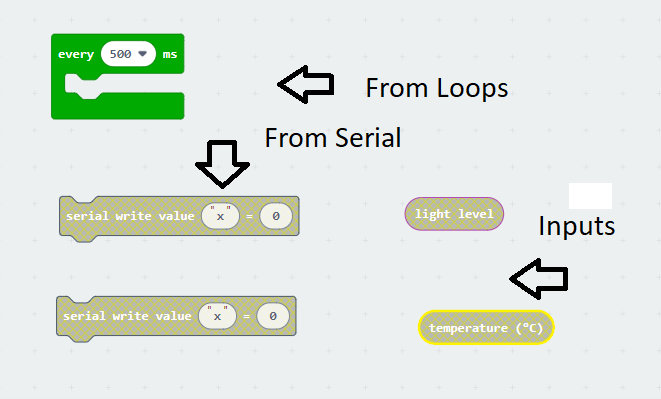
\includegraphics[width=10cm]{chapters/ChapterP2-datalog/figures/datalog2.png}
    \caption{Setting up step 1}
    \label{fig:datalogstep1}
\end{figure}


Figure 4.2 shows where various elements are in menu. To get the Serial ones you will need to open up the Advanced menu and then Serial menu options (see figure 4.3)
\begin{figure}
    \centering
    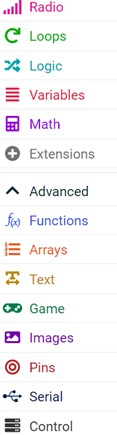
\includegraphics[width=10cm]{chapters/ChapterP2-datalog/figures/datalog3.png}
    \caption{Setting up step 2}
    \label{fig:datalogstep2}
\end{figure}
 
\begin{figure}
    \centering
    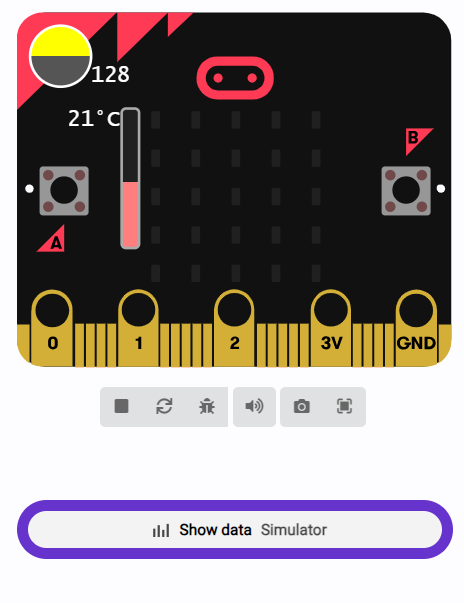
\includegraphics[width=10cm]{chapters/ChapterP2-datalog/figures/datalog4.png}
    \caption{Setting up step 3}
    \label{fig:datalogstep3}
\end{figure}

Once everything is set up under the similar microbit you will see another button “Show data Simulator” We can play with the microbit simulator toi simulate light and temperature levels; click on new data simulation button and graphs starts rolling across the screen – dag the temperature and light levels on the microbit simulator and you see the graphs change – it is logging the simulate data – it works!
Now for the fun bit.
Click on Download we need to pair the computer and microbit. Figures 4.5 to 4.8 show the steps.
 
\begin{figure}
    \centering
    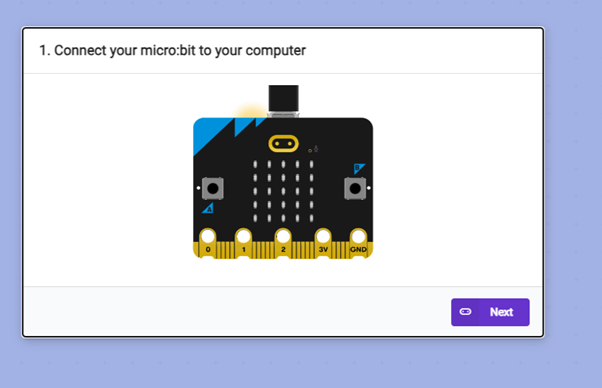
\includegraphics[width=10cm]{chapters/ChapterP2-datalog/figures/datalog5.png}
    \caption{Setting up step 4}
    \label{fig:datalogstep4}
\end{figure}
\begin{figure}
    \centering
    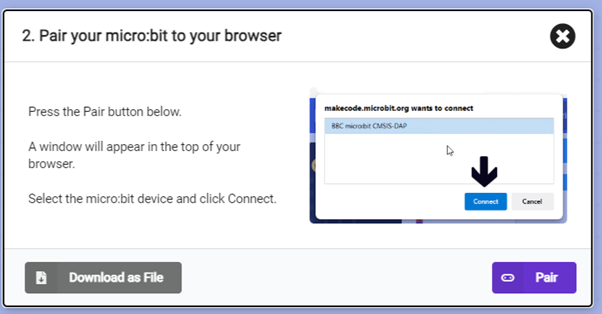
\includegraphics[width=10cm]{chapters/ChapterP2-datalog/figures/datalog6.png}
    \caption{Setting up step 5}
    \label{fig:datalogstep5}
\end{figure}

\begin{figure}
    \centering
    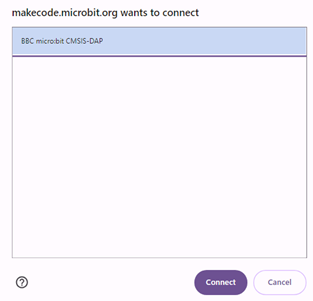
\includegraphics[width=10cm]{chapters/ChapterP2-datalog/figures/datalog7.png}
    \caption{Setting up step 6}
    \label{fig:datalogstep6}
\end{figure}
\begin{figure}
    \centering
    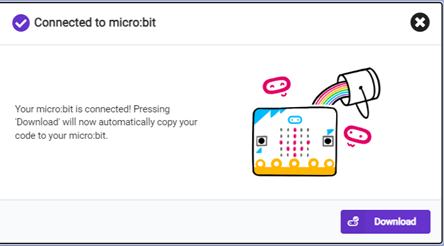
\includegraphics[width=10cm]{chapters/ChapterP2-datalog/figures/datalog8.png}
    \caption{Setting up step 7}
    \label{fig:datalogstep7}
\end{figure}

We can now take values from the real device. A new button should have appeared along with the “Show data Simulator” button; “Show data Device” Click on this button and instead os simulate data we get data from the  microbit (see figure 9)

 
\begin{figure}
    \centering
    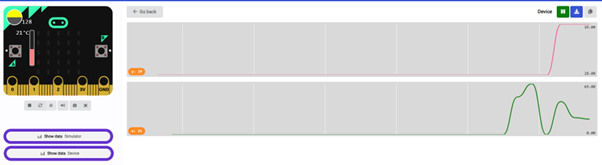
\includegraphics[width=10cm]{chapters/ChapterP2-datalog/figures/datalog9.png}
    \caption{Datalogging in action}
    \label{fig:datalogaction}
\end{figure}

So in figure 4.9 The top graph is light level the bottom is temperature taken from the room. Play with covering the sensor the LED grid and light levels change.

Collecting data is great, but we are taking it one step further logging the data over time To do this Click on the blue download button above the graphs to save the logged data as a CSV file. Once it is a CSV format it is yours to play with in other tools such as spreadsheets.


\subsection{Activity} 
-	how can this be more meaningful?
-	How do we do this with so a microbit can see data – some more remote monitoring (see \url{https://microbit.org/projects/make-it-code-it/makecode-wireless-data-logger/} )
-	How could you do this in Python?

\section{Remote sensing}

In the previous activity a single microbit was used to log data. The main problem with this is often we want to sense things that are away from the computer ie remotely (though only a short distance away). The previous solution was attached to the computer to work. So one solution (and closer to solutions used in the 'real-world' is to separate the sensing part and receiving and processing into two different devices. So in this case two micro bits; one collecting and sending data, and the other receiving and transferring the data to the computer.

\subsection{Getting started}

So to play with this, we are going to extend our previous solution to be a remote monitoring system; and the easiest way to get started is with a solution that already exists and adapt it. So we going to use the solution found in \url{https://microbit.org/projects/make-it-code-it/makecode-wireless-data-logger/} as our starting point (I would suggest literally use the makecode provided and then adapt it)

 

Advice: To avoid confusion when programming the microbits; as well as using separate makecode I would suggest programming them separately and only have one microbit at a time plugged in to the computer, to avoid confusion.

 
\subsection{Microbit 1: Transmitter and sensors}
For those that don’t know; microbit can send bits of data over short distances to and from microbits, details on how can be found at https://makecode.microbit.org/reference/radio. For this application we create a 'group' really just give the group a number, and then send our sensor values by radio.

We are going to keep sending the values, light and temperature, but not connect it to the computer directly (after programming) so the microbit in use will need a battery to power it but can be moved away from the computer - it's remote!

 

Here is the code:
\begin{figure}
    \centering
    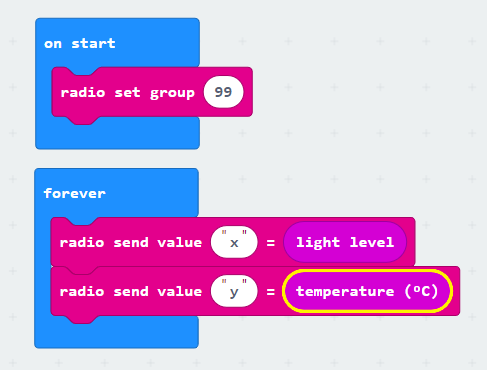
\includegraphics[width=10cm]{chapters/ChapterP2-datalog/figures/datalog10.png}
    \caption{Transmitter code}
    \label{fig:datalogtransmitter}
\end{figure}





 

 

Microbit 2: Reciever

This is the one we keep connected to the computer.

What we need to do is the following

-            Use the same radio group number as the transmitter

-            -Receive the radio signal and based on the name received (in this case x or y) allocated the value sent with the name to a variable.

-            -finally write the values to the screen (just as we did with the single microbit solution) and display them.

\begin{figure}
    \centering
    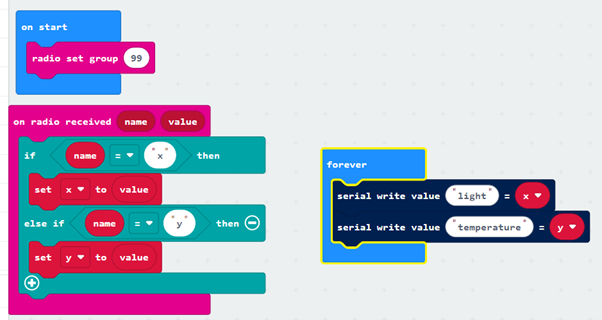
\includegraphics[width=10cm]{chapters/ChapterP2-datalog/figures/datalog11.png}
    \caption{Reciever code}
    \label{fig:datalogreciever}
\end{figure}
 
\subsection{Summary}

Essentially we have split what we did in the first activity across two microbits connected by a radio link. Running the "Show data" button on the receiver MakeCode window; as before you should get something like this.

\begin{figure}
    \centering
    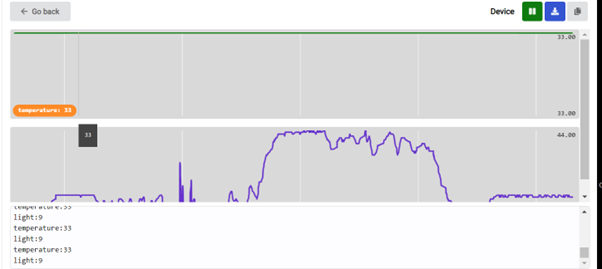
\includegraphics[width=10cm]{chapters/ChapterP2-datalog/figures/datalog12.png}
    \caption{Remote Data Logging}
    \label{fig:datalogremotedatalogging}
\end{figure}
Unless temperature is changing fairly quickly you might not see a great deal of change but hold the transmitter in your hand and you will see some changes. The light level can be made to change also be moving the transmitter so the LED array is pointed at bright screen

 

To save the data as a CSV file and view later in an spreadsheet; as before just use the blue download icon.

\subsection{Some suggestions for improvement}

-            When the two microbits are running without the graphs by just looking at the microbit, especially the transmitter, it is not clear that it is doing anything. So could something we added to fix this?

-            Play around with the sampling rate (ie. how often do you send data). So in the transmitter do what we did in the our single microbit solution, replace the forever loop with one that send data every so often.

Have fun.

